\documentclass[a4paper,11pt]{article}
\usepackage[utf8]{inputenc}
\usepackage{amsmath}
\usepackage{amsfonts}
\usepackage{amssymb}
\usepackage{graphicx}
\usepackage{braket}

\numberwithin{equation}{section}
\renewcommand\thesubsection{\alph{subsection}}
\newcommand{\bvp}[1]{\mathbf{#1}'}
\newcommand{\bv}[1]{\mathbf{#1}}
\newcommand{\ez}{\epsilon_0}
\newcommand{\lrp}[1]{\left({#1}\right)}
\newcommand{\lrb}[1]{\left\{{#1}\right\}}


%opening
\title{Computational Biology HW4}
\author{Vince Baker}

\begin{document}

\maketitle

\section{Problem 1}
i) Following the derivation in Frankel and Smit, we calculate the potential through two partial integrations.
The problem is spherically symmetric, so $\Phi$ will not depend on $\theta$ or $\phi$. 
We first rewrite $\nabla^2\Phi(r)$ in a form with a second derivative:
\begin{align}
 \lrp{\frac{1}{r^2}\frac{\partial }{\partial r}\lrp{r^2\frac{\partial}{\partial r}}}\Phi(r) &= \frac{2}{r}\frac{\partial \Phi}{\partial r}+\frac{\partial^2 \Phi}{\partial r^2} \\
 \frac{1}{r}\frac{\partial^2 }{\partial^2 r}(r\Phi) &= \frac{2}{r}\frac{\partial \Phi}{\partial r}+\frac{\partial^2 \Phi}{\partial r^2}\\
 \nabla^2\Phi(r) = \frac{1}{r}\frac{\partial^2 }{\partial^2 r}(r\Phi)
\end{align}
We now solve for $\Phi$ for a Gaussian charge distribution by two partial integrations.
\begin{align}
 \frac{1}{r}\frac{\partial^2 }{\partial^2 r}(r\Phi) &= 4\pi q_i \frac{a^3}{\ez\pi^{3/2}} e^{-a^2r^2}\\
 \frac{\partial}{\partial r}(r\Phi) &= 4\pi q_i\frac{a^3}{\ez\pi^{3/2}}\int_\infty^r dr\  re^{-a^2r^2}\\
 \frac{\partial}{\partial r}(r\Phi) &= -2 q_i\frac{a}{\ez\pi^{1/2}} e^{-a^2r^2}\\
 r\Phi &= -2 q_i\frac{a}{\ez\pi^{1/2}}\int_0^rdr\  e^{-a^2r^2}\\
 \Phi &= -\frac{q_i}{\ez r} erf(ar)
\end{align}
ii) As $r \rightarrow 0$ the potential approaches the value $-\frac{2}{\ez\sqrt{\pi}}$. 
This makes Gaussian charge distributions (relatively) easy to handle computationally as there is no singularity as there is for a delta function charge distribution.
\\
As $r\rightarrow\infty$ the Gaussian potential approaches 0. 
The error function derivative is $\propto e^{-x^2}$ so the potential rolls off faster than $\frac{1}{r^3}$, making it a short-range potential.
\\
\section{Computational experiment}
1, 2) The full $N^2$ simulation took 63.64 seconds, the truncated potential with a cutoff range of $r_c=2.5$ took 21.6 seconds. 
The faster execution time is expected, since the forces do not have to be calculated between every pair of molecules.
This improvement is less than you might naively expect, as the cutoff method still must loop through all $N(N-1)/2$ molecule pairs and calculate minimum-image distances.
\\
3) The computational time required for different Verlet skin radii is shown below, the value of rc was 2.5. 
When rl is very close to rc, the simulation is inefficient because the code will recompute the neighbor list whenever any particle moves farther than $(rl-rc)/2$.
When rl is too large there are an excessive number of particles in the neighbor list, leading to increasing computational complexity.\\
We see that the Verlet list method is generally more efficient than the simple cutoff method. Even with a poor choice of rl the execution time is still reduced by a factor of 2.
A proper choice of rl provides a full order of magnitude improvement.
\\
\begin{figure}[h]
 \caption{Impact of Verlet skin radius on computational time}
 \centering
   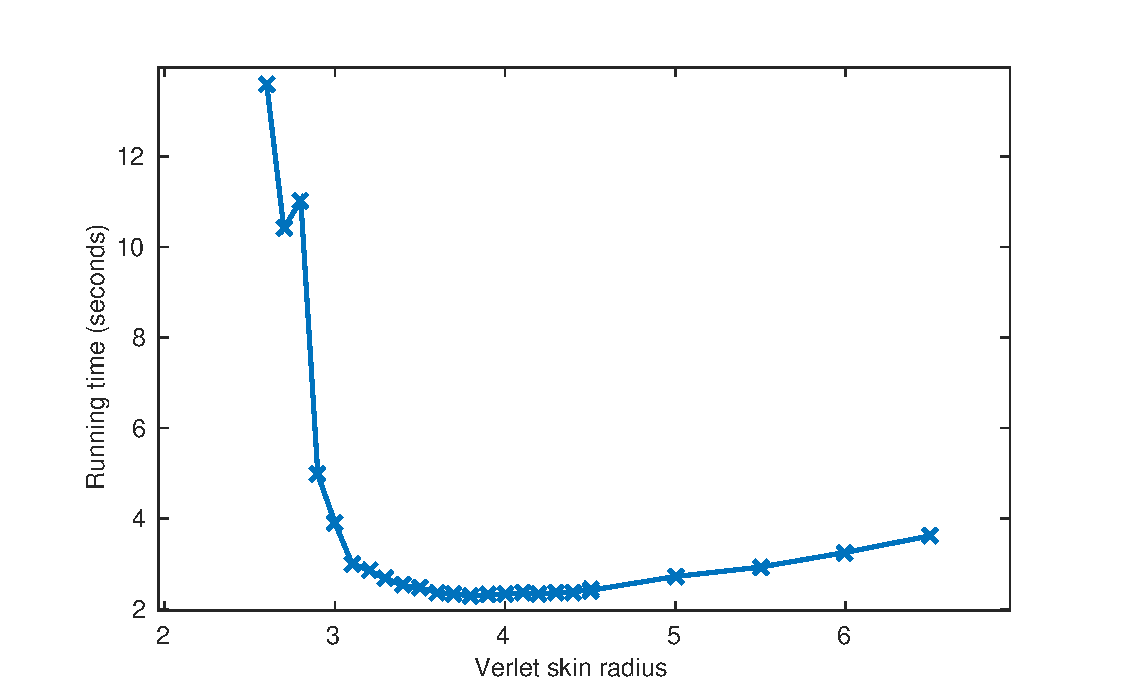
\includegraphics[width=\textwidth]{p1}
\end{figure}

\end{document}
